\question[6]1.下列说法正确的是
\begin{center}
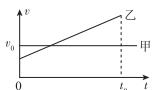
\includegraphics[]{img/image1.jpeg}
\end{center}

\fourchoices{A.加速度为正值,物体一定做加速直线运动}{B.百米比赛时,运动员的冲刺速度越大成绩越好}{C.做直线运动的物体,加速度为零时,速度不一定为零,速度为零时,加速度一定为零}{D.相对于某参考系静止的物体,对地速度不一定为零}
\begin{solution}{4cm}

\end{solution}



\question[6]密目2.小球在水中运动时受到水的阻力与小球运动速度的平方成正比,即$f=kv,$则比例系数k的单位是
\fourchoices{$kg·m^2$}{$kg·m$}{}{$kg/m^2$}
\begin{solution}{4cm}

\end{solution}



\question[6]⋮目3.正在海上行驶的一艘帆船,行驶方向如图所示,海风吹来的方向与船行驶的方向夹角为$53°,$升起风帆,调整风帆的角度,使海风垂直吹在帆面上,若海风吹在帆面上的风力大小为$500N,$则沿船行驶方向获得的推力大小为$(sin53°=0.8,cos53∘=0.6)$


\fourchoices{$300N$}{$375N$风}{目}{$400N450N$}
\begin{solution}{4cm}

\end{solution}



\question[6]4.可看作质点的甲、乙两汽车沿着两条平行车道直线行驶,在甲车匀速路过A处的同时,乙车从此处由静止匀加速启动,从某时刻开始计时,两车运动的$v━t$图象黑目如图所示$,t_b$时刻在B处甲、乙两车相遇.下面说法正确的是一甲
\begin{center}
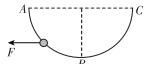
\includegraphics[]{img/image4.jpeg}
\end{center}

\fourchoices{$A.A,B$两处的距离为$v_0t_0$}{$B.t.$时刻乙车的速度是$2v_0$}{$C.t=0$时刻两车并排行驶}{$D.t=0$时刻乙车行驶在甲车前面}
\begin{solution}{4cm}

\end{solution}



\question[6]5.如图所示,木箱置于水平地面上,一轻质弹簧一端固定在木箱顶部,另一端系一小球,小球下端用细线拉紧固定在木箱底部.剪断细线,小球上下运动过程中木箱刚好不能离开地面.已知小球和木箱的质量相同,重力加速度大小为g,若$t_0$时刻木箱刚好不能离开地面,下面说法正确的是
\fourchoices{$A.t_0$时刻小球速度最大$B.t_0$时刻小球加速度为零MM}{$C.t_0$时刻就是刚剪断细线的时刻$D.t_0$时刻小球的加速度为2g}{$⋮.C.kg/m$}{⋮画}
\begin{solution}{4cm}

\end{solution}



\question[6]6.如图所示$,A,B$两个小球用长为1m的细线连接,用手拿着A球,B球竖直悬挂,且$A、B$两球均静止.现由静止释放A球,测得两球落地的时间差为$0.2s,$不计空气阻力,重力加速度$g=10m/s^2,$则A球释放时离地面的高度为
\begin{center}
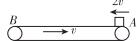
\includegraphics[]{img/image6.jpeg}
\end{center}

\fourchoices{$1.25m$}{$1.80mB●$}{}{$3.60m6.25m$}
\begin{solution}{4cm}

\end{solution}



\question[6]7.如图所示$,A、B,C,D$四个小球质量分别为$m、4m,2m、3m,$用细线连着,在A和C之间细线上还串接有一段轻弹簧,悬挂在光滑定滑轮的两边并处于静止状态.弹簧的形变在弹性限度内,叫重力加速度大小为g,则下列说法正确的是
\begin{center}
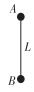
\includegraphics[]{img/image7.jpeg}
\end{center}

\fourchoices{A.剪断$C,D$间细线的一瞬间,小球C的加速度大小为3g}{B.剪断$C,D$间细线的一瞬间,小球A和B的加速度大小均为$\frac{3}{7}g$}{C.剪断$A、B$间细线的一瞬间,小球C的加速度大小为零B●}{D.剪断C球上方细线的一瞬间,小球A和B的加速度大小均为零}
\begin{solution}{4cm}

\end{solution}



\question[6]8.某人提着箱子站在电梯里,电梯从一楼上升到三楼的整个过程中先匀加速后匀减速,关于此过程,下列说法正确的是
\fourchoices{A.手对箱子的力大小始终等于箱子对手的力的大小}{B.手对箱子的力大小始终等于箱子的重力的大小}{C.人对电梯的压力先持续增大后持续减小}{D.人对电梯的压力先大于人和箱子的总重力后小于人和箱子的总重力}
\begin{solution}{4cm}

\end{solution}



\question[6]9.将一个小球竖直向上抛出,碰到高处的天花板后反弹,并竖直向下运动回到抛出点,若反弹的速度大小是碰撞前速度大小的$0.65$倍,小球上升的时间为$1s,$下落的时间为$1.2s,$重力加速度取$10m/s^2,$不计空气阻力和小球与天花板的碰撞时间,则下列说法正确的是
\begin{center}
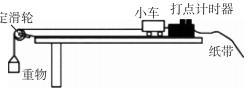
\includegraphics[]{img/image9.jpeg}
\end{center}

\fourchoices{A.小球与天花板碰撞前的速度大小为$10m/s$}{B.小球与天花板碰撞前的速度大小为$8m/s$}{C.抛出点到天花板的高度为$15m$}{D.抛出点到天花板的高度为$13m$}
\begin{solution}{4cm}

\end{solution}



\question[6]$10.$如图所示,半圆$ABC$是由一条光滑的杆弯曲而成的.带有小孔的小球穿在杆上,在水平拉力F的作用下小球由B点开始缓慢升高,此过程中半圆$ABC$竖直固定不动$,AC$连线水平.在小球缓慢上升的过程中,有关水平拉力F、杆对小球的作用力$F_N$的变化情况,下列说法正确的是
\fourchoices{F逐渐变大}{F逐渐变小}{}{$F_N$逐渐变大$F_N$逐渐变小}
\begin{solution}{4cm}

\end{solution}



\question[6]$11.$如图所示,水平传送带以大小为v的速率沿顺时针匀速运行,一个小物块从传送带的右端点A以大小为2v的速度向左滑上传送带,小物块滑到传送带正中间时速度减为零.已知小物块与传送带间的动摩擦因数为$\mu,$重力加速度为g,则下列说法正确的是
\begin{center}
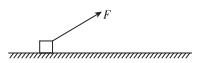
\includegraphics[]{img/image11.jpeg}
\end{center}

\fourchoices{$A.A,B$两点间的距离为$\frac{2v^{2}}{\mu g}$}{B.小物块在传送带上运动时与传送带的相对位移为$\frac{9v^{2}}{2\mu g}$}{C.要使小物块从传送带左端点B滑离,小物块在右端点A滑上传送带的速度至少为3v}{D.增大传送带的速度(仍小于$2v),$小物块与传送带间相对运动的时间变长}
\begin{solution}{4cm}

\end{solution}



\question[6]$12.$质量为m的物块放在水平桌面上,物块与水平桌面间的动摩擦因数为$\frac{\sqrt{3}}{3}$现给物块一个斜向上的拉力F使物块匀速向右运动,则拉力F的值可能为
\begin{center}
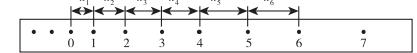
\includegraphics[]{img/image12.jpeg}
\end{center}

\fourchoices{$\frac{1}{4}mg$}{$\frac{1}{3}mg$}{}{$\frac{1}{2}mgmg$}
\begin{solution}{4cm}

\end{solution}



